1.
    \begin{figure}[h]\centering
    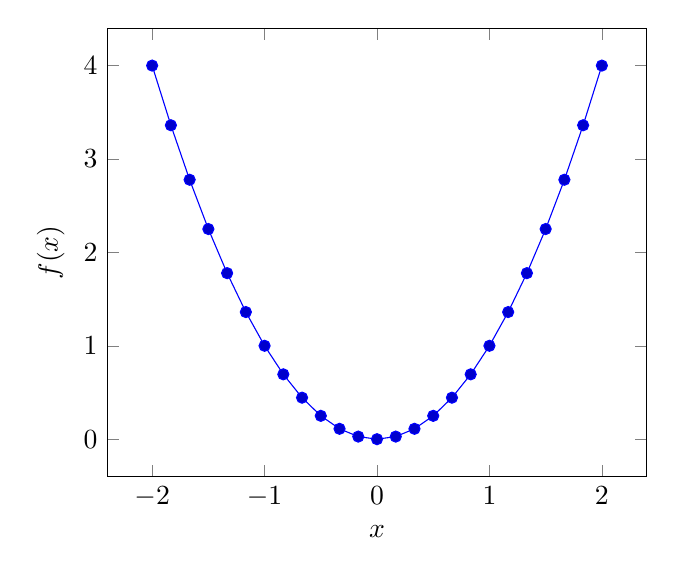
\begin{tikzpicture}
        \begin{axis}[xlabel = \(x \), ylabel = \(f(x)\), domain=-2:2]
            \addplot {x^2};
        \end{axis}
    \end{tikzpicture}
    \end{figure}

2.
    \begin{figure}[h]\centering
    \begin{tikzpicture}
        \begin{axis}[
            xlabel = \(x \), ylabel = \(f(x)\), axis lines = left, domain=0:2*pi
        ]
            \addplot[samples=150] {sin(deg(2*x))};
        \end{axis}
    \end{tikzpicture}
    \end{figure}

3. 
    \begin{figure}[h]
    \centering
    \begin{tikzpicture}
        \begin{axis}[xlabel = \(x \), ylabel = \(f(x)\)]
            \addplot[samples=150] {2/(1+exp(-2*(x-0.5)))};
            \addplot[dashed, domain=-5:0.5] {1}; 
            \draw[->] (axis cs: -2,1.5) node[above] {Mid point} -- (axis cs: 0.48,1.02);
        \end{axis}
    \end{tikzpicture}
    \end{figure}

4.
    \begin{figure}[h]\centering
    \begin{tikzpicture}
    \begin{axis}[
        xlabel=t, ylabel=y(t), title=System response,
        axis lines = middle,
        legend pos = outer north east,
        align=center, %allows multi-line text in a node
        clip=false, scale=1.3
    ]
        \addplot[blue,samples=100, domain=0:10] {1/2*(1- exp(-2*x))} ;
        \addlegendentry{$v_{out}(t)$};
        \addplot[red,thick, domain=0:10] {1};
        \addlegendentry{$v_{desired}(t)$}
        \addplot[domain=-2:0,red,thick] {0};
        \draw[->] (axis cs: 8,0.53) -- (axis cs: 8,0.98) node[midway, right](){Steady-state \\ error};
        %%Dashed lines
        \draw[dashed] (axis cs: 0.5,0) -- (axis cs: 0.5,0.32) ;
        \addplot[dashed, domain=0:0.5] {0.32};
        \addplot[dashed, domain=0:2] {0.5};
    \end{axis}
    \end{tikzpicture}
    \caption{System response given a step input}
    \end{figure}
\end{enumerate}